This chapter explains how we can use the simulator and the pieces we modelled in the preceding chapter to model a whole robot. We then showcase some simulations that were used to validate robot designs and finally present the influence these simulations had on the final design of the robot. 

\section{Overview of the simulation setup}
V-Rep is used to simulate the physics of the robot but the control code runs alongside and not inside V-Rep. This is possible because V-Rep runs a server thread which can process specific instructions\footnote{An alphabetical list of those instructions can be found on \url{http://www.coppeliarobotics.com/helpFiles/en/remoteApiFunctionListAlphabetical.htm}} sent by a client thread. This gives us great implementation flexibility and we can substitute the real robot by the simulation model easily. This is represented on \cref{fig:simulation_principles}.

\begin{figure}[htp]
\center
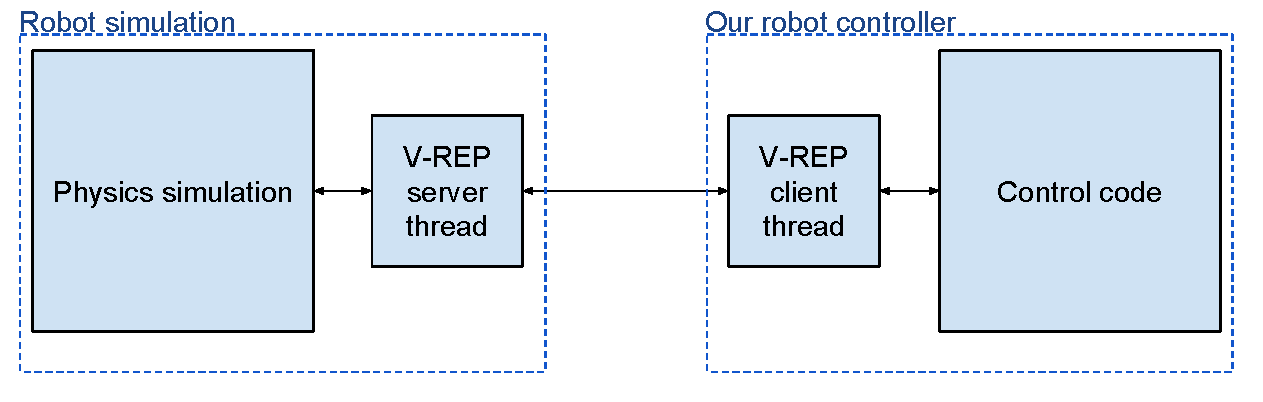
\includegraphics[width=0.7\textwidth]{figures/simulation_principles}
\caption[Simulation principles]{V-Rep simulates the robot while an external program sends order to the robot over TCP/IP thanks to the client/server thread provided by V-Rep.}
\label{fig:simulation_principles}
\end{figure}

Furthermore, the simulation will operate in the synchronous operation mode. That is, each simulation timestep must be triggered by the control code, allowing precise control of the robot. \Cref{fig:remoteApi} presents how V-Rep and the control code interact in synchronous mode.

\begin{figure}[htp]
\center
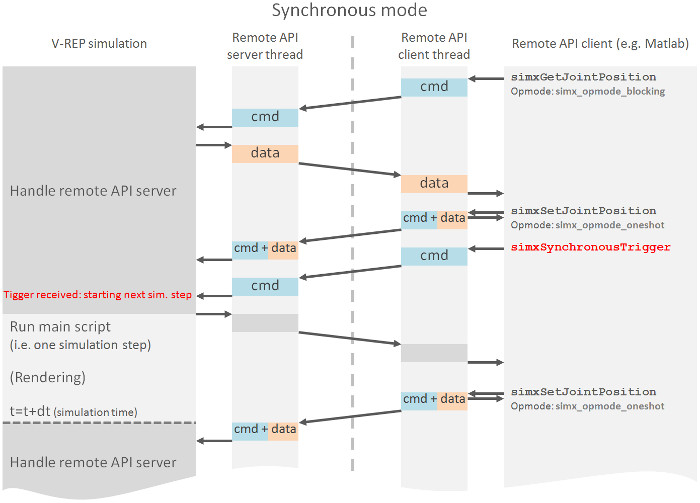
\includegraphics[width=0.8\textwidth]{figures/remoteApiSynchronous}
\caption[Simulation interaction]{Typical interaction between the simulator and the control code. The simulation runs on two threads : the simulation and the server thread. The server threads can receive orders from a client thread which is controlled by a custom application of our own. The simulator waits for a trigger before simulating the next timestep.\cite{vrep_manual}}
\label{fig:remoteApi}
\end{figure}

The instructions available can execute a number of different actions. The following proved most useful for this project :\begin{itemize}
\item simxGetObjectHandle : this function is used to retrieve a handle on an object. A handle is necessary if a user wants to perform operations on an object.
\item simxSetJointTargetPosition : this function sets a target position for a joint.
\item simxSetFloatSignal : this function gives the possibility of setting the value of a signal inside V-Rep. A signal is a variable created during the simulation that is accessible both to the simulator and the external world. This is useful if we want to extend the interface that V-Rep provides.
\item simxGetFloatSignal : this function retrieves the value of a float signal. 
\end{itemize}

\section{Applications}
\subsection{Static stability}
The first application is simply to build a model of the robot and test if it is able to stand upright on its own, using the servos. That model is presented in \cref{fig:robotv7}

The servos of the robot are simply ordered to hold their initial angle and the simulation determines that the robot can indeed stand upright without any active stabilization. This is a simple test that can rule out bad designs quite easily.

\subsection{Going from a supine to a prone lying position}
The main motivation for a routine that makes the robot move from a supine\footnote{lying on the back} lying position to a prone\footnote{lying on the belly} one is that it allows us to only have one standing up routine. 

The routine is defined as follows :\begin{enumerate}
\item From $0$ to $0.39sec$ : the robot brings his right arm above his head while preparing the left one to lift its body from the left side. Both legs are twisted towards the right side at the hips.

\item From $0.40$ to $0.99sec$ : the left leg swings towards the right side while the right leg swings towards the left side. The left elbow prepares to push.

\item From $1.00$ to $1.59sec$ : the left elbow pushes the body up and the hips untwist. The left feet touches the ground on the right side.

\item At $1.6sec$ : The robot relaxes all its limbs and is now prone.
\end{enumerate}

The evolution of the angles held by the joints during the routine is presented in \cref{fig:sup2proneArms} and \cref{fig:sup2proneLegs}. 

\begin{figure}[htp]
\center
    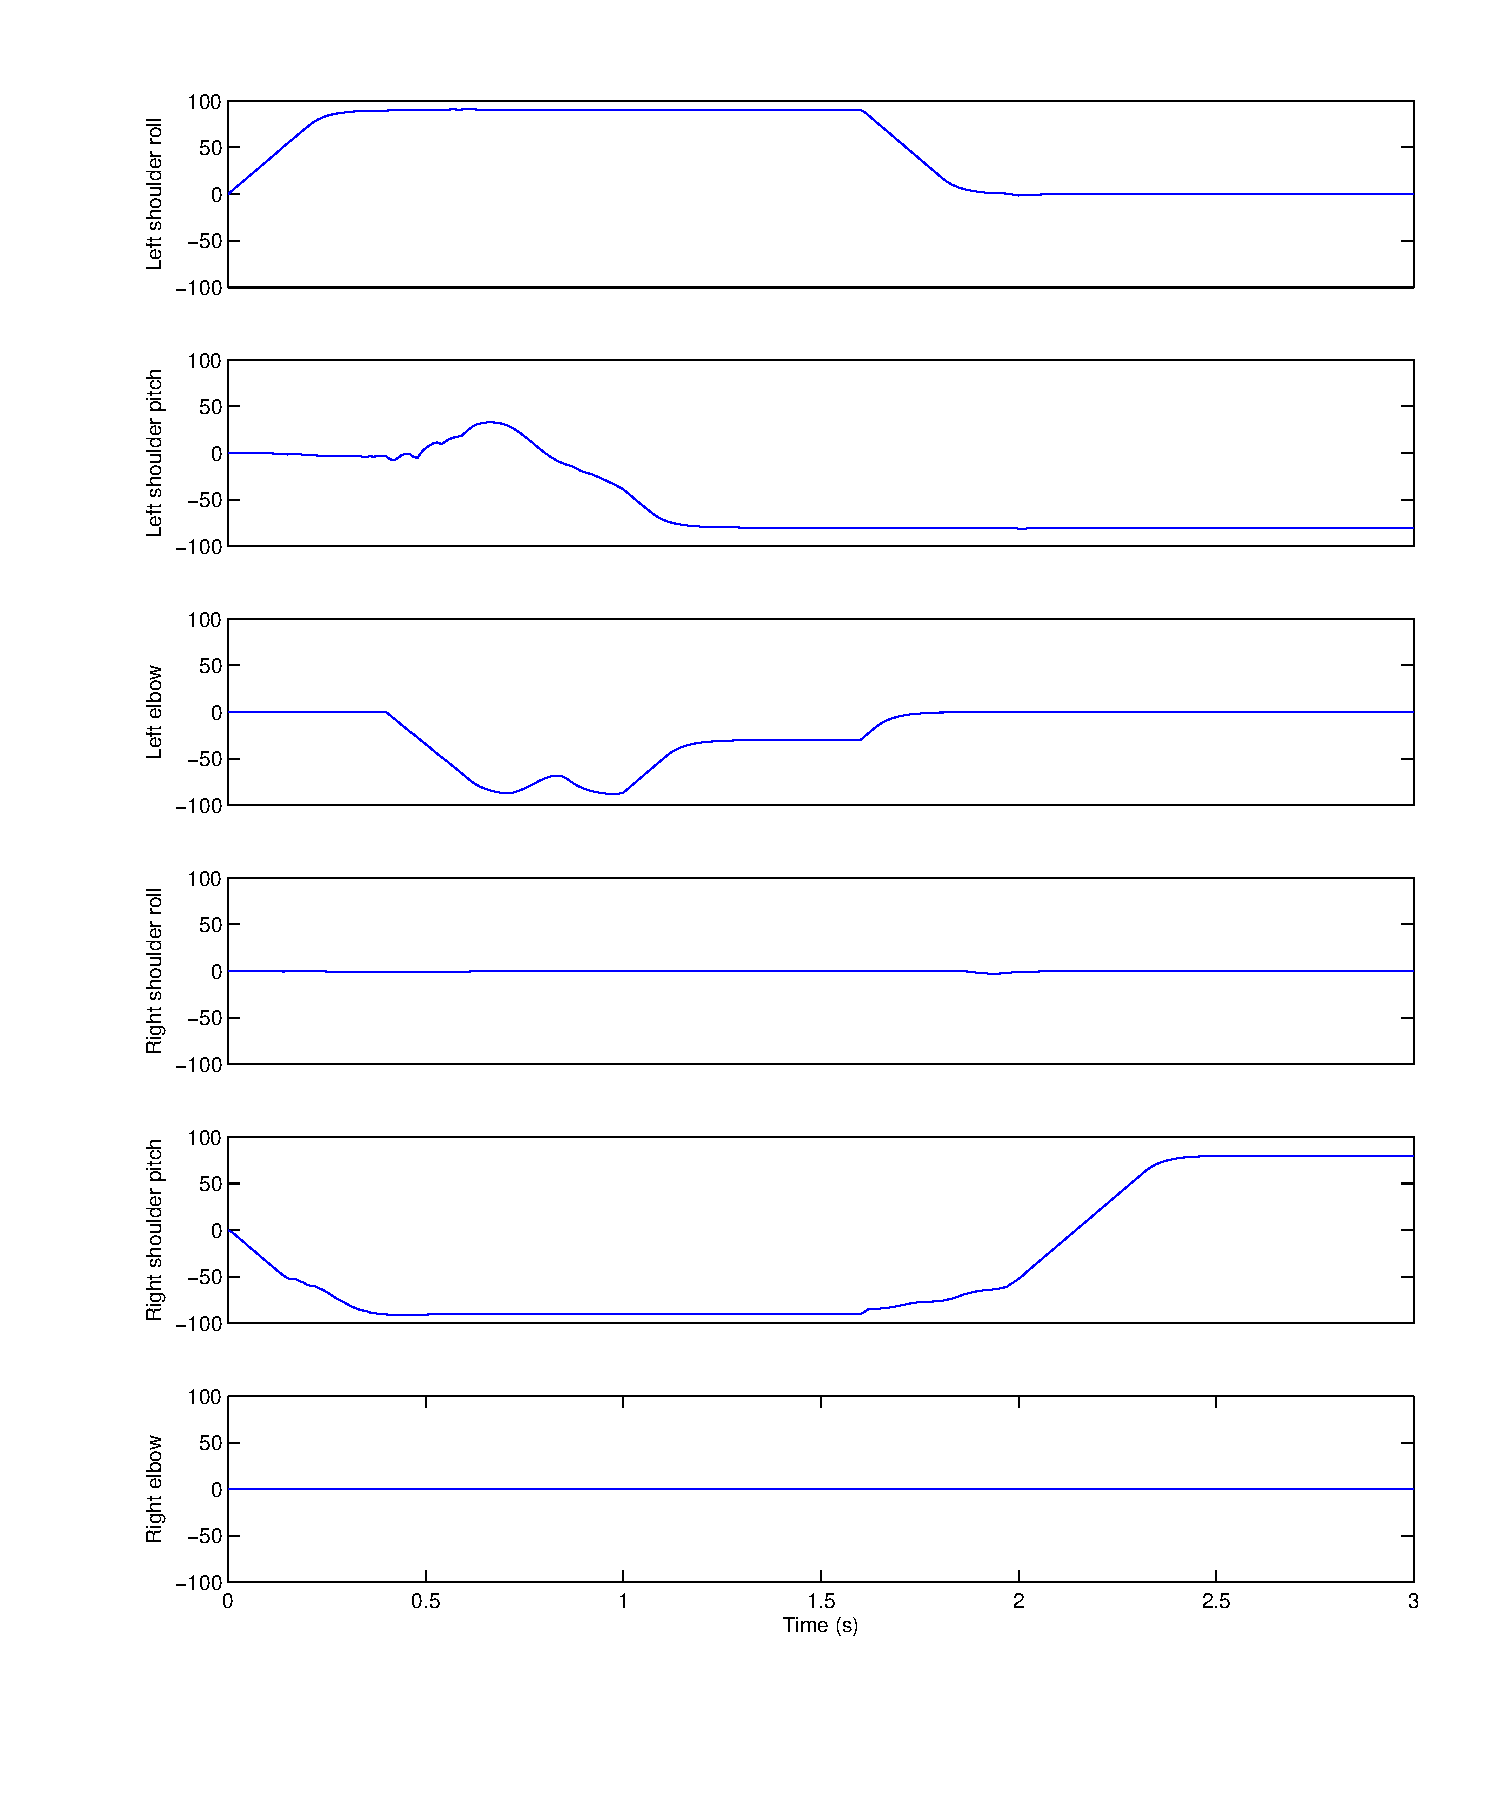
\includegraphics[width = \textwidth]{figures/sup2proneArms}
    \caption[Angles of the arms during \emph{supine} to prone manoeuvre]{Angles of the arms during \emph{supine} to prone manoeuvre. Predictably it is the left arm that is the most active as it is the one that is used to make the robot roll over. We notice that at times (around $0.7sec$) the left elbow does not generate enough torque to hold the desired angle.}
    \label{fig:sup2proneArms}
\end{figure}

\begin{figure}[htp]
\center
    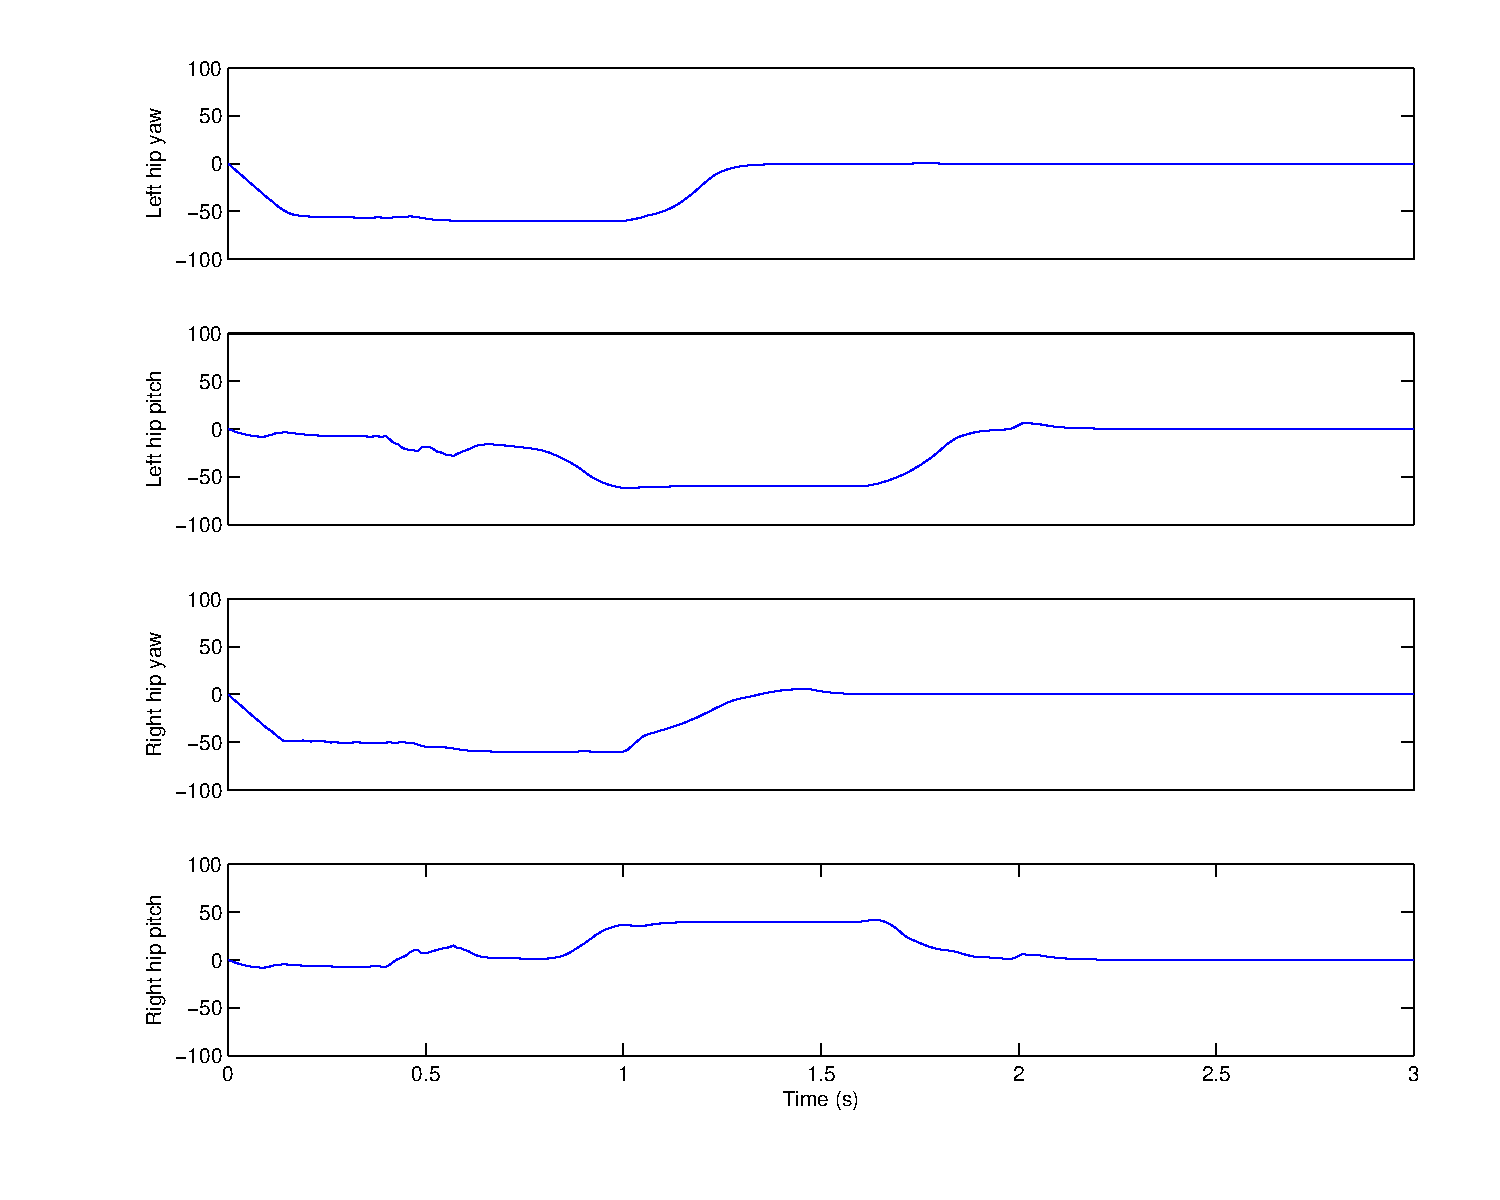
\includegraphics[width = \textwidth]{figures/sup2proneLegs}
    \caption[Angles of the legs during \emph{supine to prone} manoeuvre]{Angles of the legs during \emph{supine to prone} manoeuvre.}
    \label{fig:sup2proneLegs}
\end{figure}

\subsection{Standing up from a prone lying position}
This routine was inspired by Jörg Stückler, Johannes Schwenk, and Sven Behnke in \cite{Stuckler06}. It is defined as follows:\begin{enumerate}
\item From $0.00$ to $0.19sec$ : in preparation for the arms to lift the body in the next step we adjust the roll of the shoulders.

\item From $0.20$ to $0.49sec$ : in order to reduce the stress on the servos of the arm, we bend the arms a little before the next step.

\item From $0.50$ to $0.89sec$ : lift the body up through the hips with the help of the arms. This step and the next are preparation for the next step where we will move the feet underneath the body.

\item From $0.90$ to $1.39sec$ : now that the body is held up by the arms we reverse the holding angle for the hips, to move the hips up. 

\item From $1.40$ to $1.99sec$ :  we move the feet underneath the body by bending the knees and bringing the legs closer to the body. The objective is to bring the center of mass inside the support area of the feet.

\item From $2.80$ to $4.00sec$ : the robot slowly gets up by unbending the knees and the hips. 
\end{enumerate}

\begin{figure}[htp]
\center
    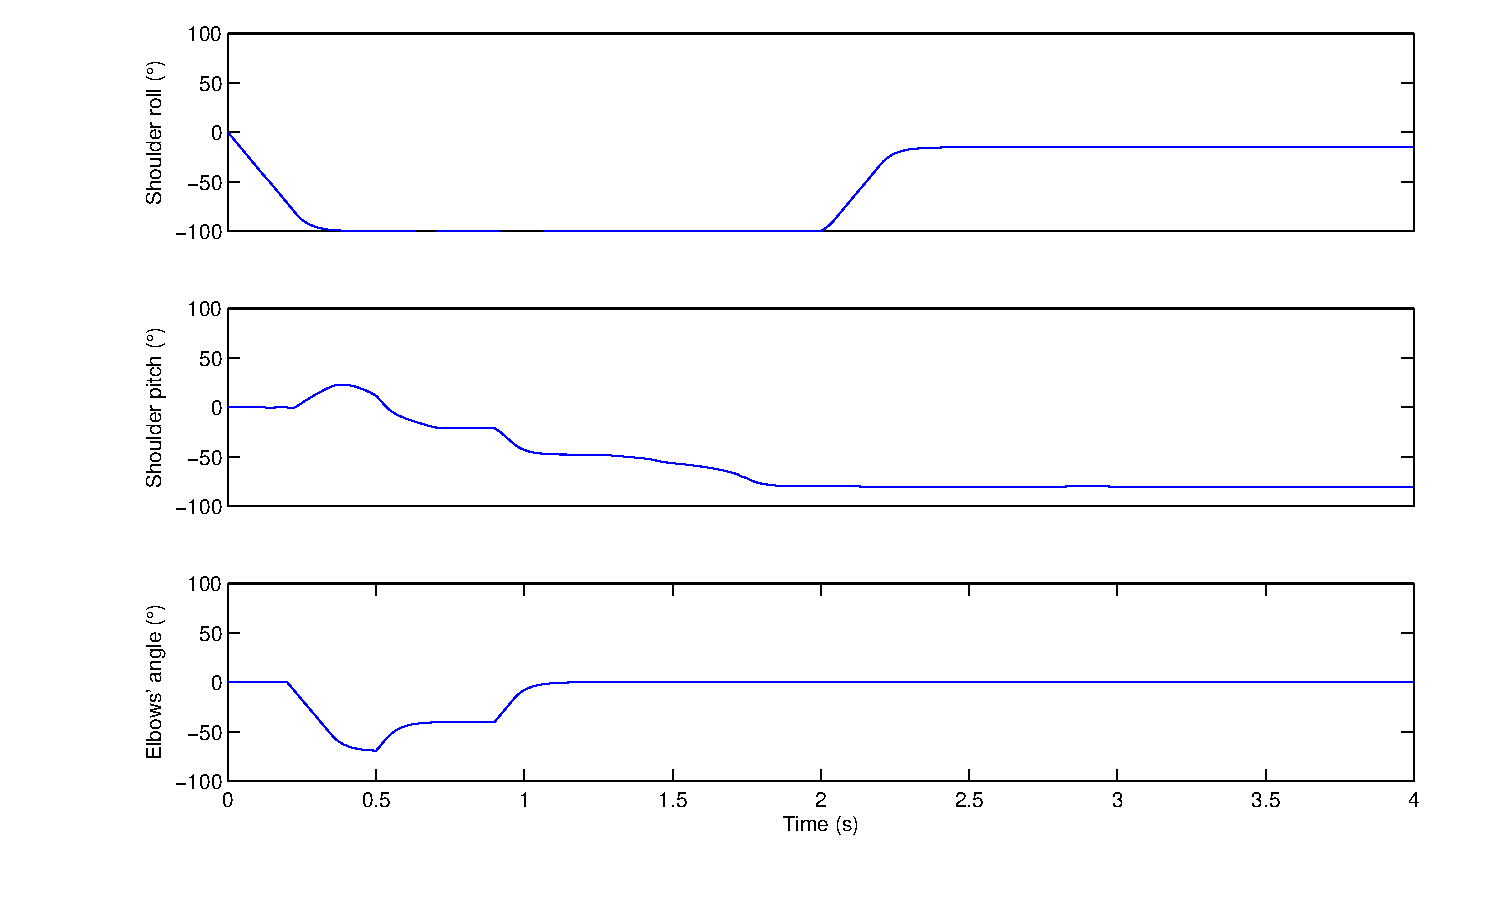
\includegraphics[width = \textwidth]{figures/prone2standArms}
    \caption[Angles of the arms during \emph{supine} to prone manoeuvre]{Angles of the arms during \emph{supine} to prone manoeuvre}
    \label{fig:prone2standArms}
\end{figure}

\begin{figure}[htp]
\center
    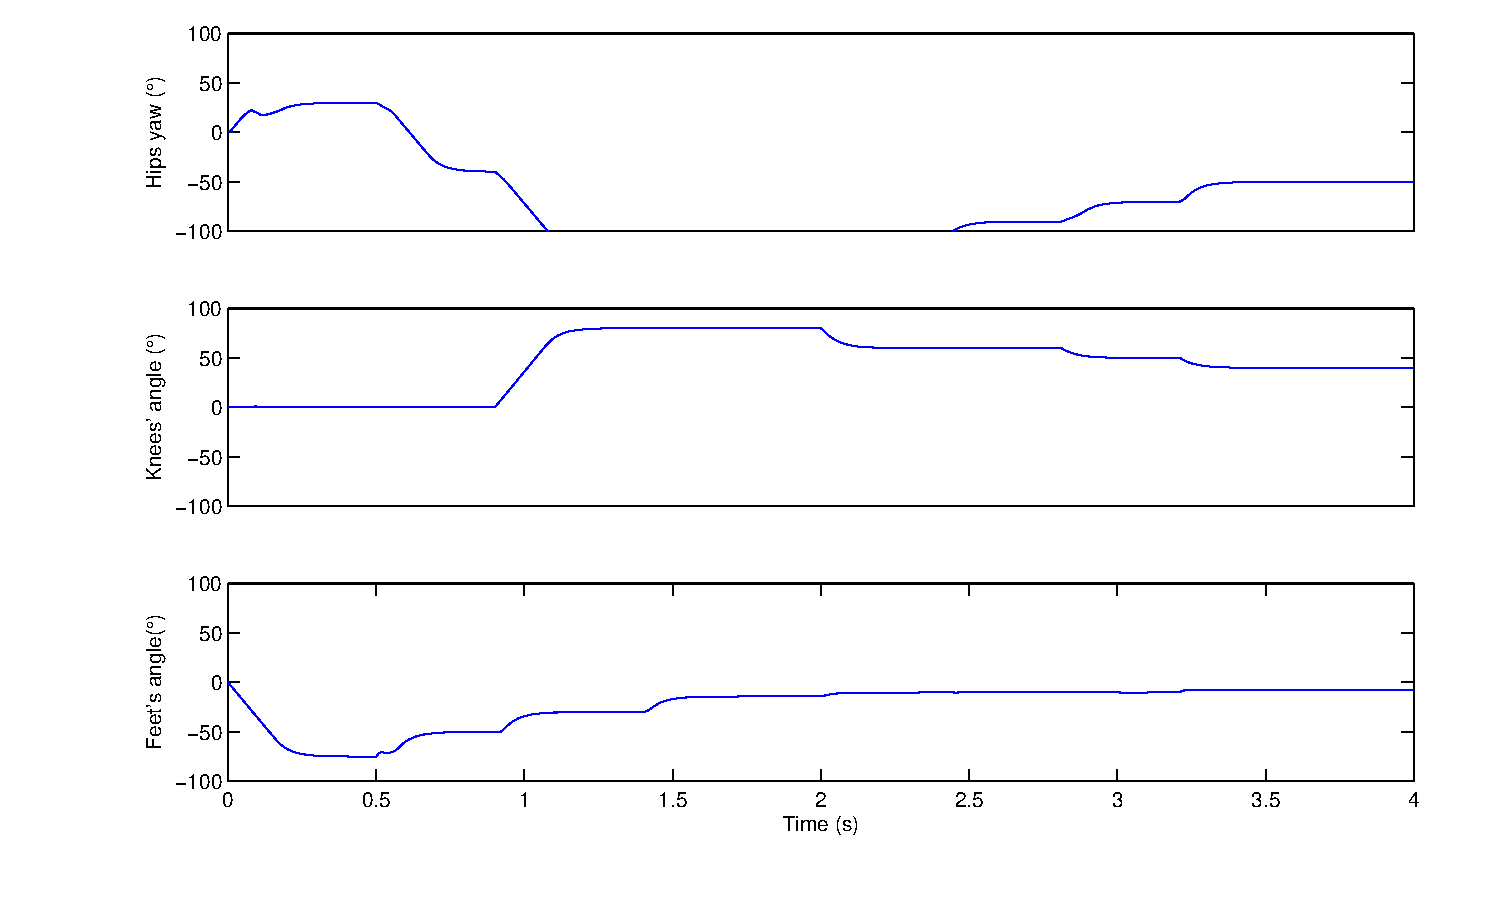
\includegraphics[width = \textwidth]{figures/prone2standLegs}
    \caption[Angles of the legs during \emph{supine to prone} manoeuvre]{Angles of the legs during \emph{supine to prone} manoeuvre}
    \label{fig:prone2standLegs}
\end{figure}

\section{Influence of the simulations on the final design of the robot}
The simulator helped shape the robot through simulations that unveiled serious design problems (inability to stand after a fall, inability to walk).

The first design is visible on \cref{fig:first_robot}. It was plagued by stability problems, overcomplicated arms and simulation difficulties. 
\begin{figure}[htp]
\center
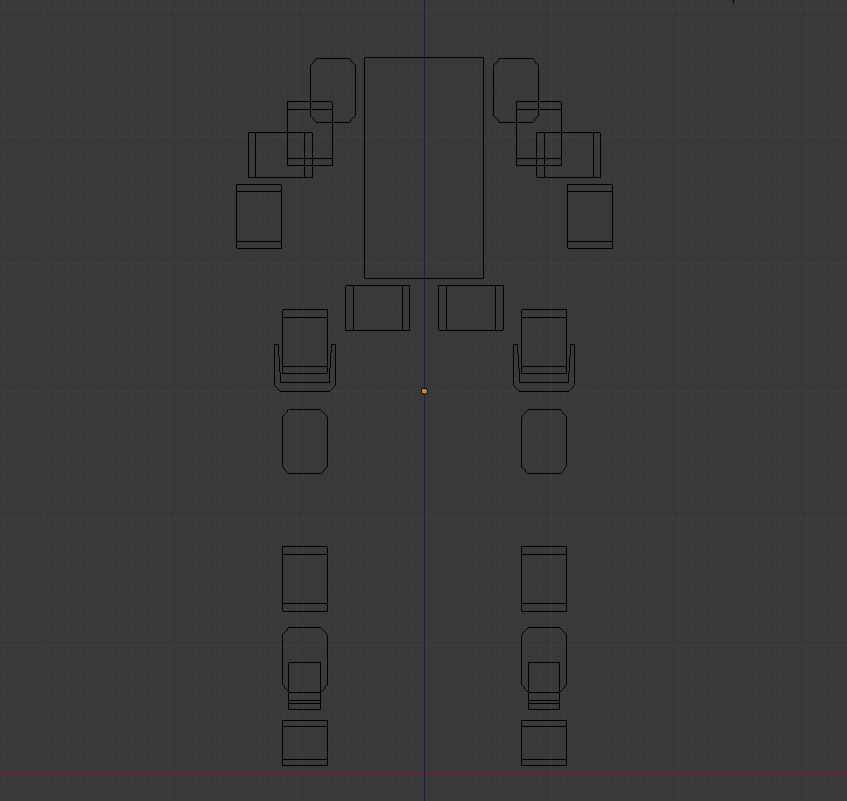
\includegraphics[width=0.6\textwidth]{figures/robot1}
\caption[Initial robot design]{First robot design. Each arm is made of 4 servos, making them quite heavy.}
\label{fig:first_robot}
\end{figure}

The final design, visible on \cref{fig:final_robot} has better stability, wider movement possibilities and can stand up and walk more easily. 
\begin{figure}[htp]
\center
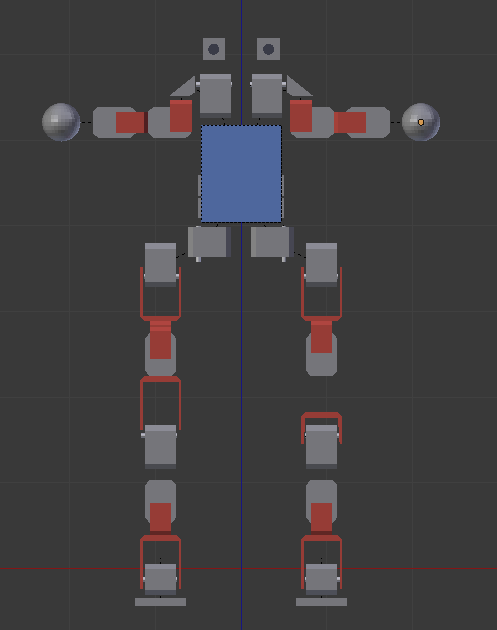
\includegraphics[width=0.6\textwidth]{figures/robot2}
\caption[Final robot design]{Final robot design. Arms now use 3 servos. The feet and the hips use a different configuration to have wider movement possibilities and bring down the center of gravity.}
\label{fig:final_robot}
\end{figure}

The final dimensions of the robot abide by the rules of the contest (see \cref{appendix:rules}) :
\begin{enumerate}
\item Height ($H_{top}$) :  $40 \leq 61.75 \leq 90cm$.
\item Weight : $2.726kg$
\item Height of center of mass ($H_{COM}$) : $34cm$. Foot area : $175 < cm^2$.
\item Foot aspect ratio : $1.79 \leq 2.5$.
\item Minimal width of the robot : $20 \leq 33.96cm$
\item $69.72 \leq 74.10cm$
\item Maximal height : $75.52 < 92.63cm$.
\item Leg length ($H_{leg}$) : $21.61 \leq 27.5 \leq 43.23cm$
\item Height of the head ($H_{Head}$) : $3.09 \leq 10.75 \leq 15.44cm$
\end{enumerate}